\chapter{Система координат}\label{cha:coordinate_system}
Нам потрібна система координат для опису зображення.
Cистема координат, що використовується для розміщення елементів по відношенню один до одного, називається користувацьким простором, оскільки це координати, які користувач використовує для визначення елементів і розташування їх по відношенню один до одного.
Система координат, використана для відображення графіки (наприклад механізм рендерінгу для Android та iOS платформ), має початок у верхньому лівому куті, вісь x простягається праворуч, а вісь y - вниз.

\begin{figure}
    \label{fig:image2}
    \centering
    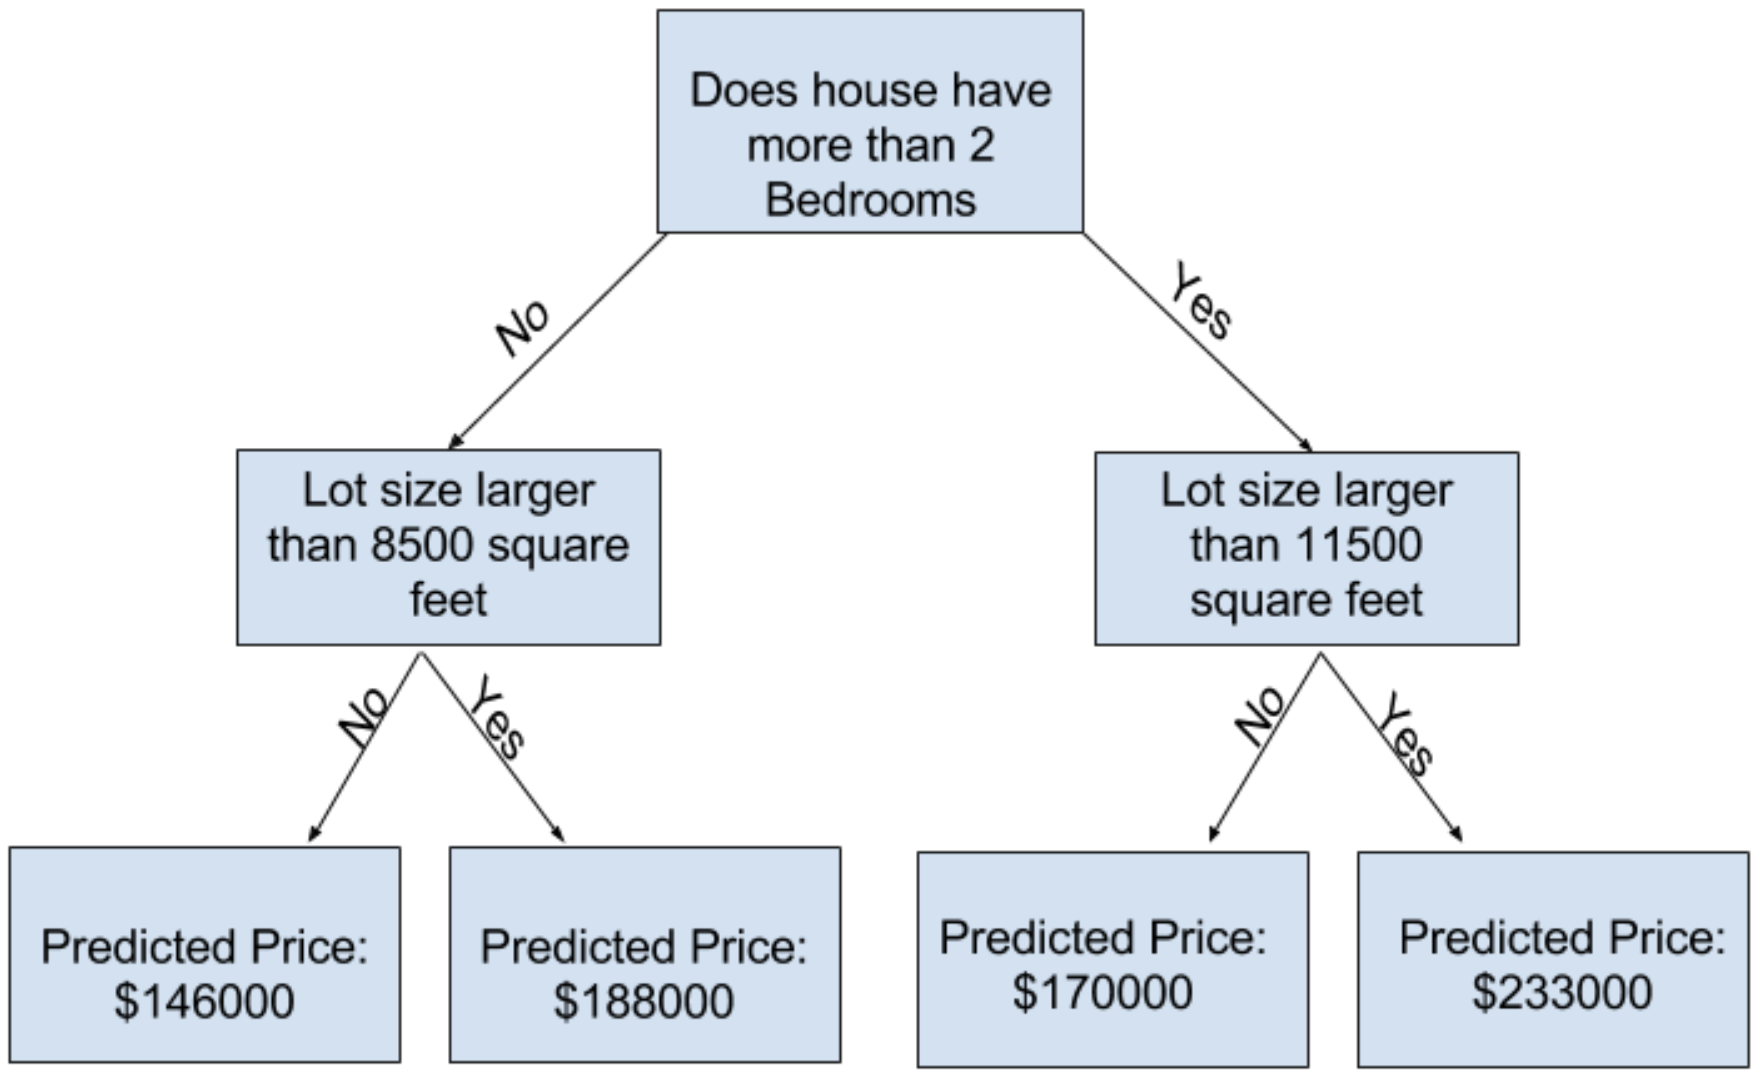
\includegraphics[scale=0.5]{image2.png}

    Рис. 2. Система координат.
\end{figure}

\pagebreak

